\documentclass{article}
\usepackage[includeheadfoot,left=1in, right=0.5in, top=0.5in, bottom=0.5in]{geometry}
\usepackage{fancyhdr}
\usepackage{lastpage}
\usepackage{extramarks}
\usepackage[usenames,dvipsnames]{color}
\usepackage{graphicx}
\usepackage[table]{xcolor}
\usepackage{listings}
%\usepackage{courier}
\usepackage{float}
\usepackage{url}
\usepackage{caption}
\usepackage[pdfborder={0 0 0}]{hyperref}
%\usepackage[compact,small]{titlesec}
\usepackage{microtype}
\usepackage{verbatim}
\usepackage{booktabs}
\usepackage{indentfirst}
\usepackage{pdfpages}
\usepackage{tabularx}

\definecolor{lightgray}{gray}{0.9}

\parskip = 0.5\baselineskip
\setlength{\belowcaptionskip}{-\baselineskip}

\captionsetup{font=scriptsize}
\captionsetup{labelfont=bf}

\pagestyle{fancy}
\rhead{Max Thrun \& Xiaohui Qi}
\lhead{EECE6080 - Intranex}
\lfoot{Progress Report 1}
\rfoot{Page\ \thepage\ of \protect\pageref{LastPage}}
\cfoot{}
\renewcommand\headrulewidth{0.4pt}
\renewcommand\footrulewidth{0.4pt}

% make verbatim text small
\makeatletter
\g@addto@macro\@verbatim\small
\makeatother

\setlength\parindent{0pt} % Removes all indentation from paragraphs

\definecolor{sh_comment}{rgb}{0.12, 0.38, 0.18 } %adjusted, in Eclipse: {0.25, 0.42, 0.30 } = #3F6A4D
\definecolor{sh_keyword}{rgb}{0.37, 0.08, 0.25}  % #5F1441
\definecolor{sh_string}{rgb}{0.06, 0.10, 0.98} % #101AF9

\lstset{
    language=vhdl,
    xleftmargin=.25in,
    xrightmargin=.25in,
    numbers=left,
    numberstyle=\tiny,
    frame=tb,
    showstringspaces=false,
    captionpos=b,
    stringstyle=\color{sh_string},
    keywordstyle = \color{sh_keyword}\bfseries,
    commentstyle=\color{sh_comment}\itshape,
    basicstyle=\small\sffamily,
    %numbersep=-5pt,
    belowskip=\baselineskip,
    aboveskip=\baselineskip
}

\begin{document}

\includepdf{../cover_page/cover_page.pdf}
\newpage
\tableofcontents
\newpage
\listoffigures
\listoftables
\lstlistoflistings
\newpage
\section{Pinout Diagram}

\begin{figure}[H]
    \centering
    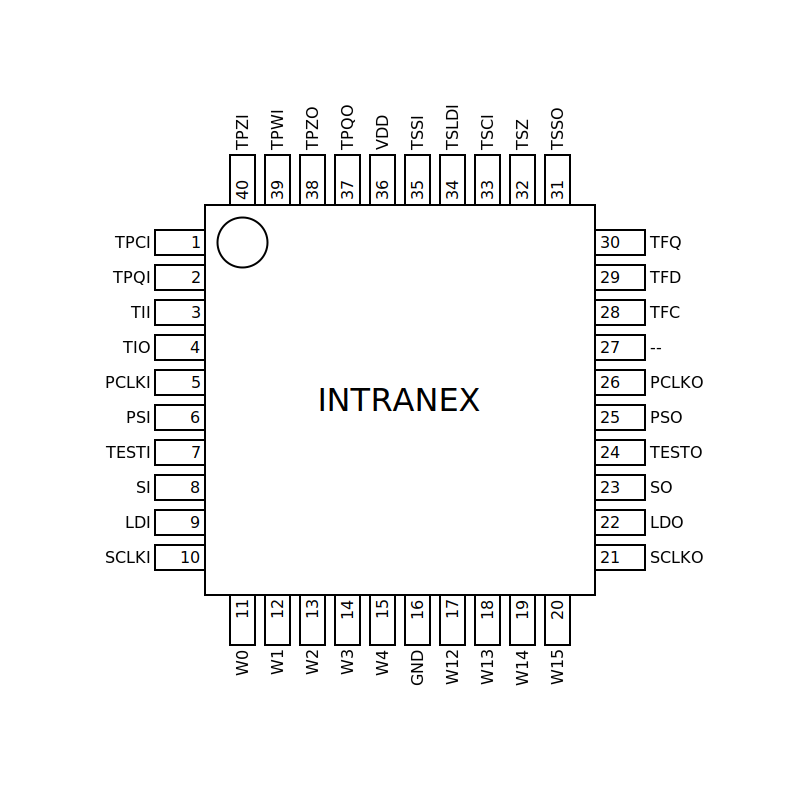
\includegraphics[width=\linewidth]{../pinout/pinout.png}
    \caption{Pinout Diagram}
\end{figure}

\begin{table}[H]
    \begin{tabularx}{\textwidth}{|l|l|c|X|}
        \hline
        \textbf{Pin \#} & \textbf{Name} & \textbf{Type} & \textbf{Description} \\
        \hline
        









%
%
%
%
%
%
%
%
%
%
% MAIN PINS
% TEST DFF
% TEST INVERTER
% TEST PIN SLICE
% TEST SHIFT SLICE
1  & TPZO   & O & Test pin slice row output \\ \hline
2  & TPZI   & I & Test pin slice row input \\ \hline
3 & TII   & I & Test inverter input \\ \hline
4 & TIO   & O & Test interter output \\ \hline
5  & PCLKI & I & PIN clock input \\ \hline
6  & PSI   & I & PIN serial input \\ \hline
7  & TESTI & I & Test Mode enable input\\ \hline
8  & SI    & I & Serial input \\ \hline
9  & LDI   & I & Parallel load input \\ \hline
10 & SCLKI & I & Serial clock input \\ \hline
11 & W0 & O & W0 Debug Output \\ \hline
12 & W1 & O & W0 Debug Output \\ \hline
13 & W2 & O & W0 Debug Output \\ \hline
14 & W3 & O & W0 Debug Output \\ \hline
15 & W4 & O & W0 Debug Output \\ \hline
16 & GND   & P & -- \\ \hline
17 & W12 & O & W0 Debug Output \\ \hline
18 & W13 & O & W0 Debug Output \\ \hline
19 & W14 & O & W0 Debug Output \\ \hline
20 & W15 & O & W0 Debug Output \\ \hline
21 & SCLKO & O & Serial clock output \\ \hline
22 & LDO   & O & Parallel load output \\ \hline
23 & SO    & O & Serial output \\ \hline
24 & TESTO & O & Test Mode enable output\\ \hline
25 & PSO   & O & PIN serial output \\ \hline
26 & PCLKO & O & PIN clock output \\ \hline
28 & TFQ   & O & Test flop-flop Q output \\ \hline
29 & TFC   & I & Test flip-flop clock input \\ \hline
30 & TFD   & I & Test flip-flop D input \\ \hline
31 & TSSO  & O & Test shift slice serial output \\ \hline
32 & TSZ   & I & Test shift slice parallel input \\ \hline
33 & TSSI  & I & Test shift slice serial input \\ \hline
34 & TSLI  & I & Test shift slice load input \\ \hline
35 & TSCI  & I & Test shift slice clock input \\ \hline
36 & VDD   & P & -- \\ \hline
37 & TPWI   & I & Test pin slice coloumn \\ \hline
38 & TPQO   & O & Test pin slice serial output \\ \hline
39 & TPQI   & I & Test pin slice serial input \\ \hline
40 & TPCI   & I & Test pin slice clock input \\ \hline

    \end{tabularx}
    \caption{Pin Descriptions}
\end{table}

\newpage
\section{Chip Functionality}

\subsection{Configuring the Programmable Interconnect Network}
\begin{figure}[H]
    \centering
    \includegraphics[width=\linewidth]{../waveforms/pin.png}
    \caption{PIN Configuration}
\end{figure}

\subsection{Loading and reading a value}
\begin{figure}[H]
    \centering
    \includegraphics[width=\linewidth]{../waveforms/shift_load.png}
    \caption{Loading a value}
\end{figure}

\begin{figure}[H]
    \centering
    \includegraphics[width=\linewidth]{../waveforms/shift_load_read.png}
    \caption{Loading a value and reading the result}
\end{figure}

\subsection{Test Mode}

\begin{figure}[H]
    \centering
    \includegraphics[width=\linewidth]{../waveforms/test.png}
    \caption{Enabling test mode and loading all DFFs}
\end{figure}

\section{Design Decisions}

\section{Block Diagrams}

    \subsection{Top Level}

    \begin{figure}[H]
        \centering
        \includegraphics[width=\linewidth]{../../logisim/top.png}
        \caption{Top Level Block Diagram (3-Bit Configuration)}
    \end{figure}

    \subsection{Parallel Load Shift Register}

        \subsubsection{Bit-slicing Scheme}
        \begin{figure}[H]
            \centering
            \includegraphics[width=\linewidth]{../../logisim/shift.png}
            \caption{Parallel Load Bit-Sliced Shifter Register (3-Bit Configuration)}
        \end{figure}

        \subsubsection{Bit-Slice}
        \begin{figure}[H]
            \centering
            \includegraphics[width=\linewidth]{../../logisim/shift_slice_mux.png}
            \caption{Parallel Load Shifter Register Bit-Slice}
        \end{figure}

    \subsection{Programmable Interconnect Network}

        \subsubsection{Bit-slicing Scheme}
        \begin{figure}[H]
            \centering
            \includegraphics[width=\linewidth]{../../logisim/pin.png}
            \caption{Bit-Sliced Programmable Interconnect Network (3-Bit Configuration)}
        \end{figure}

        \subsubsection{Bit-Slice}
        \begin{figure}[H]
            \centering
            \includegraphics[width=\linewidth]{../../logisim/pin_slice.png}
            \caption{Programmable Interconnect Network Bit-Slice}
        \end{figure}


\section{VHDL Models}
\subsection{Top Level}
\subsection{PIN}
\lstinputlisting[caption=PIN VHDL Module]{../../vhdl/pin.vhd}
\subsection{PIN Slice}
\lstinputlisting[caption=PIN Slice VHDL Module]{../../vhdl/pin_slice.vhd}
\subsection{Shifter}
\lstinputlisting[caption=Parallel Load Shifter VHDL Module]{../../vhdl/shift.vhd}
\subsection{Shifter Slice}
\lstinputlisting[caption=Parallel Load Shifter Slice VHDL Module]{../../vhdl/shift_slice.vhd}
\subsection{Gates}
\lstinputlisting[caption=AOI21X1 VHDL Module]{../../vhdl/aoi21x1.vhd}
\lstinputlisting[caption=DFFPOSX1 VHDL Module]{../../vhdl/dffposx1.vhd}
\lstinputlisting[caption=INVX1 VHDL Module]{../../vhdl/invx1.vhd}
\lstinputlisting[caption=MUX2X1 VHDL Module]{../../vhdl/mux2x1.vhd}

\section{VHDL Test Benches}
\subsection{Top Level}
\subsection{PIN}
\subsection{PIN Slice}
\lstinputlisting[caption=PIN Slice VHDL Test Bench]{../../vhdl/pin_slice_tb.vhd}
\subsection{Shifter}
\subsection{Shifter Slice}
\lstinputlisting[caption=Parallel Load Shifter Slice VHDL Test Bench]{../../vhdl/shift_slice_tb.vhd}

\section{Work Division}

\end{document}
